\hypertarget{introducciuxf3n}{%
\section{Introducción}\label{introducciuxf3n}}

\begin{frame}{Introducción}

La demodulación de AM es el proceso inverso de modulación de AM. Un
receptor convencional de AM de doble banda lateral tan sólo reconvierte
una onda de amplitud modulada a la información de la fuente original.
Para hacerlo, el receptor debe ser capaz de recibir, amplificar y
demodular una onda de AM. También debe ser capaz de limitar la banda del
espectro total de radiofrecuencias a determinada banda deseada de
frecuencias. El proceso de selección se llama sintonía del receptor.

\end{frame}

\hypertarget{paruxe1metros-del-receptor}{%
\section{Parámetros del receptor}\label{paruxe1metros-del-receptor}}

\begin{frame}{Parámetros del receptor}

Hay varios parámetros de uso común para evaluar las posibilidades de un
receptor para demodular bien una señal de radio. Los más importantes son
la selectividad y la sensibilidad, que se usan con frecuencia para
comparar la calidad de dos radiorreceptores.

\begin{figure}
\centering
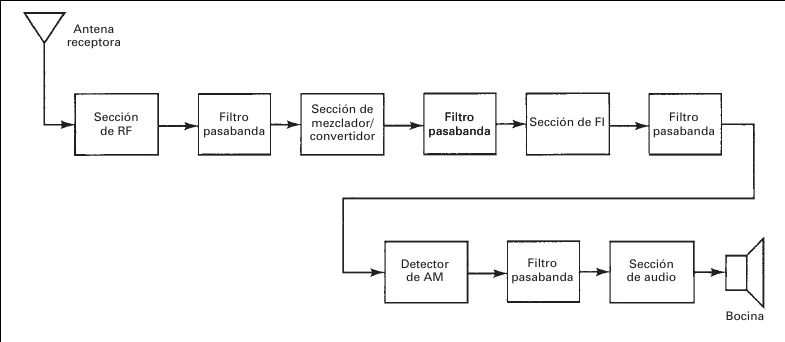
\includegraphics{DiagramaReceptorAM.png}
\caption{Diagrama de bloques simplificado de un receptor de AM}
\end{figure}

\end{frame}

\begin{frame}{Selectividad}
\protect\hypertarget{selectividad}{}

La selectividad es un parámetro del receptor con el que se mide la
capacidad de éste para aceptar una determinada banda de frecuencias y
rechazar las demás.

Hay varias formas aceptables de describir la selectividad de un receptor
de radio. Una forma frecuente es simplemente especificar el ancho de
banda del receptor en los puntos de -3 dB. Sin embargo, este ancho de
banda no es necesariamente una buena forma de determinar lo bien que el
receptor rechaza las frecuencias no deseadas. En consecuencia, se
acostumbra especificar el ancho de banda en dos niveles de atenuación,
por ejemplo, -3 dB y -60 dB. La relación de esos dos anchos de banda se
llama factor de forma, y se define con la siguiente ecuación

\[ SF = \frac{B_{-60dB}}{{B_{-3dB}}} \]

en donde:

\[ SF = \text{factor de forma (adimensional)} \]
\[ B_{-60dB} = \text{ancho de banda 60 dB abajo del nivel máximo de la señal} \]
\[ B_{-60dB} = \text{ancho de banda 3 dB abajo del nivel máximo de la señal} \]

\end{frame}

\begin{frame}{Mejoramiento del ancho de banda}
\protect\hypertarget{mejoramiento-del-ancho-de-banda}{}

El ruido térmico es la forma más prevaleciente de ruido, y es
directamente proporcional al ancho de banda. En consecuen- cia, si se
puede reducir el ancho de banda, el ruido también se reducirá en la
misma proporción y aumentará la relación de potencias de señal a ruido,
y mejorará la eficiencia del sistema. Na- turalmente hay un límite de la
eficiencia del sistema respecto a lo que se puede reducir el ancho de
banda. La relación de señal a ruido en la entrada se calcula en el
frente de un receptor, usando el ancho de banda de RF para medir la
potencia del ruido. La re- lación de reducción de ruido alcanzada
reduciendo el ancho de banda se llama mejoramiento del ancho de banda
(BI, de bandwidth improvement) y se define matemáticamente como sigue

\[BI = \frac{B_{RF}}{B_{IF}}\]

en donde:

\[BI = \text{mejoramiento del ancho de banda (adimensional)}\]
\[B_{RF} = \text{ancho de banda de RF (hertz)}\]
\[B_{IF} = \text{ancho de banda de FI (heartz)}\]

La reducción correspondiente de ruido debida a la reducción de ancho de
banda se llama mejo- ramiento de la cifra de ruido y se expresa en dB
como sigue

\[NF_{ \text{mejoramiento}} = 10 \log 20 = 30 dB\]

\end{frame}

\begin{frame}{Sensibilidad}
\protect\hypertarget{sensibilidad}{}

La sensibilidad de un receptor es el nivel mínimo de la señal de RF que
se puede detectar a la entrada del receptor y producir una señal útil de
información demodulada. La sensibilidad de un receptor de AM depende de
la potencia de ruido presente en la entrada al receptor, la cifra de
ruido (indicación del ruido generado en el frente del receptor), la sen-
sibilidad del detector de AM y el factor de mejoramiento de ancho de
banda del receptor. La mejor manera de mejorar la sensibilidad de un
receptor es reducir el nivel de ruido.

\end{frame}

\begin{frame}{Margen dinámico}
\protect\hypertarget{margen-dinuxe1mico}{}

El margen dinámico de un receptor se define como la diferencia en
decibeles entre el nivel de entrada mínimo necesario para discernir una
señal, y el valor de entrada que sobreexcita, o sa- tura, al receptor, y
produce distorsión. En términos sencillos, el margen dinámico es el
interva- lo de potencias de entrada dentro del cual el receptor es útil.

\end{frame}

\begin{frame}{Fidelidad}
\protect\hypertarget{fidelidad}{}

La fidelidad es una medida de la capacidad de un sistema de
comunicaciones para producir, a la salida del receptor, una réplica
exacta de la información de la fuente original.

\begin{figure}
\centering
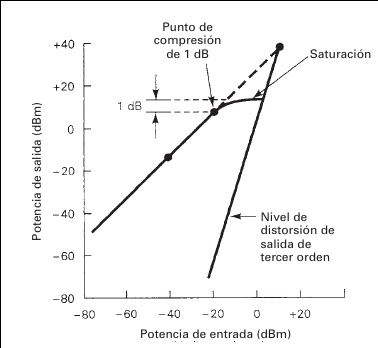
\includegraphics{fidelidad.png}
\caption{Ganancia lineal, punto de compresión de 1 dB y distorsión de
unterección de tercer orden en un amplificador normal}
\end{figure}

\end{frame}

\begin{frame}{Pérdida de inserción}
\protect\hypertarget{puxe9rdida-de-inserciuxf3n}{}

\end{frame}

\hypertarget{receptor-de-am}{%
\section{Receptor de AM}\label{receptor-de-am}}

\begin{frame}{Receptor de radiofrecuencia sintonizada}
\protect\hypertarget{receptor-de-radiofrecuencia-sintonizada}{}

\end{frame}

\begin{frame}{Receptor superheterodino}
\protect\hypertarget{receptor-superheterodino}{}

\end{frame}

\hypertarget{circuitos-receptores-de-am}{%
\section{Circuitos receptores de AM}\label{circuitos-receptores-de-am}}

\begin{frame}{Circuitos amplificadores de RF}
\protect\hypertarget{circuitos-amplificadores-de-rf}{}

\end{frame}

\begin{frame}{Circuitos de mezclador/convertidor}
\protect\hypertarget{circuitos-de-mezcladorconvertidor}{}

\end{frame}

\begin{frame}{Circuitos amplificadores de FI}
\protect\hypertarget{circuitos-amplificadores-de-fi}{}

\end{frame}

\begin{frame}{Circuitos detectores de AM}
\protect\hypertarget{circuitos-detectores-de-am}{}

\end{frame}

\begin{frame}{Controles automáticos de ganancia}
\protect\hypertarget{controles-automuxe1ticos-de-ganancia}{}

\end{frame}

\begin{frame}{Circuitos de reducción de ruido}
\protect\hypertarget{circuitos-de-reducciuxf3n-de-ruido}{}

\end{frame}

\begin{frame}{Limitadores y eliminadores de ruido}
\protect\hypertarget{limitadores-y-eliminadores-de-ruido}{}

\end{frame}

\begin{frame}{Medidas Alternas de señal de ruido}
\protect\hypertarget{medidas-alternas-de-seuxf1al-de-ruido}{}

\end{frame}

\begin{frame}{Receptores de AM en circuito integrado lineal}
\protect\hypertarget{receptores-de-am-en-circuito-integrado-lineal}{}

--\textgreater{}

\end{frame}
